\documentclass{article}
\usepackage{graphicx}
\usepackage{amsmath}

\title{Project Design}
%\subtitle{SOGM project plan, Blok 2}
\author{Akke Houben}
\date{01-03-2015}

\begin{document}
\maketitle
\section{Introduction}
\begin{figure}
	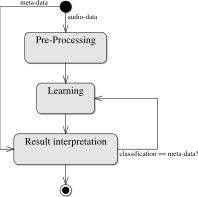
\includegraphics{plan_tot.jpg}
	\caption{Total plan of the system}
	\label{fig:total}
\end{figure}
At first the goal will be stated quickly: The goal is to create a computational model to investigate the plausibility of the Shared Sound Category Learning Mechanisms Hypothesis. The program wil consist of 3 major parts: 
\begin{enumerate}
	\item an input processing stage mimicking cochlear and cortical processing mechanisms; 
	\item a machine learning/neural network to learn sound categorization and; 
	\item a test-trial-scheduler which will feed sounds to the system, acquires the responses and displays them in a sensible way.
\end{enumerate}
The design is separated into three major parts, depicted in Figure \ref{fig:total} The first part is the 'pre-processing phase', here the incoming audio will be processed and transformed in suitable input for the 'learning phase'. The second part is the Artificial Neural Network, of which will account for the actual 'learning phase'. The third part is the test-trial scheduler, but this will -for now- not be imlemented in this project-phase.

\section{Pre-Processing Phase}
The preprocessing phase will consist of -again- two stages, following mainly the methods used by Chi, Ru and Shamma (Chi, Ru \& Shamma, 2005). The first will follow the auditory pathway from the Cochlea, trough the Auditory Nerves and trough a Lateral Inhibitory Network (LIN). The output of this stage is first integrated over a short window, to account for a futher loss of phase locking. In the second stage the Spectro-Temporal Response Fields (STFRs) of the neurons in the Primary Auditory Cortex (A1) will be modelled. The outputs of these will serve as the input to the 'learning phase'.

\begin{figure}
	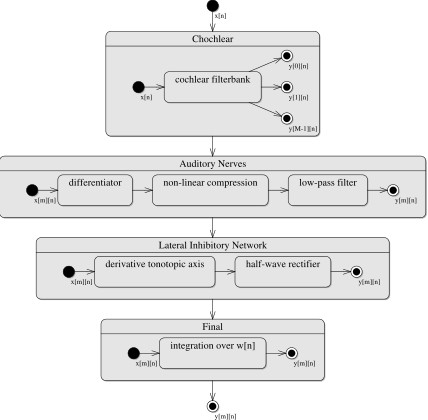
\includegraphics{stage1.jpg}
	\caption{Pre-processing phase}
	\label{fig:stage1_1}
\end{figure}

\subsection{Early Auditory Pathway}
The first stage will folow the early auditory pathway form the Cochlea, trough the Auditory Nerves end the Lateral Inhibitory Network. In Figure \ref{fig:stage1_1} a schematic representation of the processing utilized in this stage is given.
\subsubsection{Cochlear Filterbank}
The function of the Chochlea can be viewed as a parallel bank of filters (Yang et al., 1992). The audio is separated into $M$ frequency bands by a bank of gammatone filters mimicking the tonotopic filtering on the Basilar Membrane. The impulse response of the gammatone filters are given by the following equation:
\begin{equation*}
h[m][n] = an^{v-1}e^{-qn}e^{j2\pi f_{c} n}
\end{equation*}
Where:
\begin{itemize}
	\item  $a$ is the amplitude; 
	\item $v$ is the filter order (for human auditory filters a 4th order is common (Strahl, S., 2009); 
	\item $f_{c}$ is the center frequency and;
	\item $q$ is the bandwidth, mostly given by: $2\pi b ERB(cf)$
	\begin{itemize}
		\item Where $b$ is usually 1.019 for human auditory modelling (Strahl, S., 2009) and;
		\item $ERB(cf)$ is the equivalent reqtangular bandwidth at frequency $cf$ given by: $ERB(cf) = 24.7 + 1.108 cf$
	\end{itemize}
\end{itemize}
This transforms the unidimensional audio signal into a two dimensional spectrogram showing the pressure variations in separate frequency bands.

\subsubsection{Auditory Nerves}
The $M$ audio signals of this two dimensional array are independently passed trough a system mimicking the effects of the transduction of the signals trough the Auditory Nerves. Here a cascading system of a simple differentiator, a non-linear compression and a low-pass filter is implemented. The differantiator is simply the first order derivative of the individual signals with respect to the time index. The low-pass filters is a simple sinc-filter, a convolution of the signal with a sinc function:
\begin{equation*}
	w[n] = \frac{sin(2\pi f_{c} n)}{(2\pi f_{c} n)}
\end{equation*}
Where:
\begin{itemize}
	\item $f_{c}$ is the cutoff frequency
\end{itemize}

The non-linear compression is implemented using the following equation (from Yang et al., 1992): 
\begin{equation*}
	y[n] = \frac{1}{1 + e^{-g x[n]}} - \frac{1}{2}
\end{equation*}
Where:
\begin{itemize}
	\item g is the gain factor.
\end{itemize}

\subsubsection{Lateral Inhibitory Network}
The signals are then passed trough a Lateral Inhibitory Network (LIN). This LIN serves to suppress the 'excitation' of the 'neurons' next to the 'peaking-neurons'. Thus further narrowing the position on the tonotopic axis where the maximal excitation is located (??, ????).
In this model the processes are severely simplified, as Chi, Ru and Shamma (2005) also state, but are sufficient for a first version. This is a clear point of improvement for further investigation.
First the derivative of the signal along the tonotopic (frequency) axis is taken.
\begin{equation*}
    \vec{y}[m] = \frac{\delta \vec{x}[m]}{\delta m}
\end{equation*}

Then a simple half wave rectifier is applied:
\begin{equation*}
    y[n] = \frac{\sqrt{x[n]^{2}} + x[n]}{2}
\end{equation*}

\subsubsection{Final}
To finish the processing of this stage the signals are integrated over a short window $w$ to account for the further loss of phase locking in the midbrain (Chi, T., Powen, R. \& Shamma, S.A., 2005)
\begin{equation*}
    w[n] = e^{-n/\tau} u[n]
\end{equation*}
Where:
\begin{itemize}
    \item $\tau$ is a time constant ($\approx 8ms$)
\end{itemize}


\subsection{Spectro-Temporal Response Fields}
\begin{figure}
	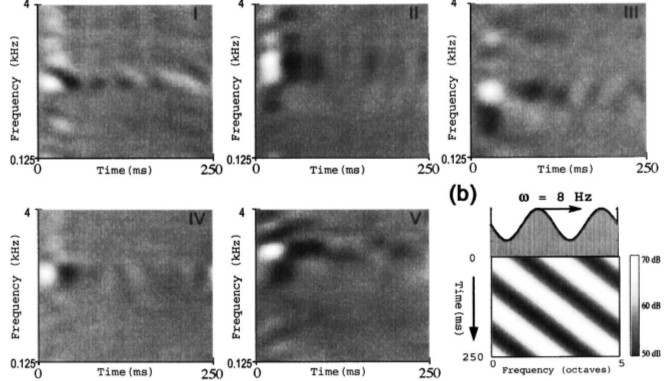
\includegraphics[width=\linewidth]{strfs.jpg}
	\caption{STRFs recorded from A1 of ferrets (taken from Chi, Ru \& Shamma (2005))}
	\label{fig:strfs}
\end{figure}
In this stage the responses of the neurons in the Primary Auditory Cortex (A1) are modelled. In several sensory pathways certain neurons react to stimuli with a specific spectro-temporal characteristic. Figure \ref{fig:strfs} shows STRFs recorded form A1 of ferrets. This functionality is simulated using a bank of filters which are selective to specific spectro-temporal patterns. 
\subsubsection{Obtaining Coefficients}
The coeficients of these STRFs will, for this implementation, probably be obtained by taking multiple affine wavelet transforms of the outputs of the first stage (Early Auditory Pathway) when several example speech sounds are used as input.
The specific method used will be clarified in a later stage.
\subsubsection{Implementation}
The specific method used will be clarified in a later stage.

\section{Learning Phase}
In this phase the actual learning will take place. An Artificial Neural Network will be modelled which will take the outputs of the STRFs neurons of the preceding section as input and will output a classification of the input as either \emph{speech} or \emph{non-speech}.
\subsection{Implementation}
The specific type of Neural Network, the design and implementation will be elaborated on in a later stage. Probably a ART-2 network will be used.

\section{Scheduler}
Finally, a system will be made which will input a corpus of sound to the system. The audio-data is put into the Pre-Processing and Learning system. The meta-data is forwarded to a result checking system, which will either serve as a \emph{feedback} for the Learning phase or which will save the classification of the Neural Network and the expected outcome. 

\subsection{Implementation}
The specific implementation will be described at a later stage.	

\end{document}
